\section{Results}
\label{sec:results}

\begin{table*}[t]
\centering
\caption{\textbf{Locked test set $\C$} (PSMA PET/CT, 125 patients; 119 tumour-positive, 4,518 lesions). Each arm was hash-locked before $\C$ was read and run once.
$\Delta$Dice: paired difference to the zero-shot system with 95\% bootstrap interval.
Harmed: patients harmed relative to the system deployed at that level (Eq.~\ref{eq:harm}), with the exact one-sided 95\% upper bound (UB) on the harm rate.
Level 1 is certified at $\delta=0.05$; Level 2 at $\delta=0.10$ (at the pre-registered $\delta=0.05$ the switch was refused and the system rolled back to the Level-1 output; \cref{sec:main}).
Best certified result in \textbf{bold}.}
\label{tab:main}
\setlength{\tabcolsep}{5pt}
\small
\begin{tabular}{@{}lccccccc@{}}
\toprule
arm & cert. & Dice $\uparrow$ & \makecell{$\Delta$Dice vs.\ zero-shot\\{\scriptsize[95\% CI]}} & \makecell{FP\\mL $\downarrow$} & \makecell{lesions\\det.\ $\uparrow$} & \makecell{HD95\\mm $\downarrow$} & \makecell{harmed / 125\\(UB) $\downarrow$} \\
\midrule
zero-shot segmenter & -- & 0.107 & -- & 733.9 & 2092 & 198.0 & -- \\
\midrule
\multicolumn{8}{@{}l}{\emph{Level 1: refinement-agent updates} (reference: deployed agent $f_0$)} \\
deployed agent $f_0$ & -- & 0.109 & $+0.002$ {\scriptsize[$+0.000$, $+0.004$]} & 719.2 & 2094 & 198.0 & -- \\
naive self-improvement & \xmark & 0.236 & $+0.129$ {\scriptsize[$+0.094$, $+0.170$]} & 196.1 & 2074 & 147.1 & 11 (14.1\%) \\
pseudo-label self-training & \xmark & 0.108 & $+0.001$ {\scriptsize[$-0.001$, $+0.003$]} & 739.9 & 2094 & 198.2 & \phantom{0}4 (7.2\%) \\
\ours, uncalibrated & \cmark & 0.129 & $+0.022$ {\scriptsize[$+0.010$, $+0.037$]} & 505.1 & 2093 & 194.3 & \phantom{0}1 (3.7\%) \\
\ours (deployed as $f_1$) & \cmark & 0.116 & $+0.009$ {\scriptsize[$+0.004$, $+0.015$]} & 592.4 & 2094 & 194.0 & \phantom{0}0 (2.4\%) \\
\midrule
\multicolumn{8}{@{}l}{\emph{Level 2: segmenter update} (reference: Level-1 system $f_1$)} \\
\ours: fine-tuned segmenter & \cmark & \textbf{0.547} & $\mathbf{+0.440}$ {\scriptsize[$+0.396$, $+0.484$]} & \textbf{14.5} & \textbf{3547} & 90.9 & \phantom{0}3 (6.1\%) \\
\ours: fine-tuned + agent & \cmark & \textbf{0.549} & $+0.442$ {\scriptsize[$+0.398$, $+0.486$]} & \textbf{14.3} & 3530 & \textbf{75.9} & \phantom{0}3 (6.1\%) \\
\bottomrule
\end{tabular}
\end{table*}

\subsection{Zero-shot transfer is safe but poor}
\label{sec:zeroshot}
Transferred unchanged, the source segmenter reaches Dice 0.10 on PSMA and predicts 732\,mL of false-positive volume per scan, most of it physiological uptake in salivary glands, kidneys and bladder (\cref{fig:qual}).
The source-domain agent, also frozen, harms no one---0 of 377 patients (95\% UB 0.8\%)---but changes Dice by only $+0.001$.
A refinement agent built on FDG cannot repair a segmenter that was never shown PSMA; the system must change.

\subsection{Main result}
\label{sec:main}
\Cref{tab:main} reports every arm on the locked test set.

\para{Level 1: certified agent updates are safe and small.}
On $\B$, LTT certified 22 of the 88 agent updates (all with zero harmed patients on $\B$); the deployed one (calibrated detector, gate 0.97, both guards) adds 63 actions on $\C$.
On the locked test it harms none of the 125 patients ($p=0.0016$ against $R>0.05$; UB 2.4\%), loses no lesion, cuts FP volume by 127\,mL per scan ($[-186,-74]$; $-18\%$) and improves Dice over the deployed agent by $+0.0068$ ($[+0.0022,+0.0126]$, $p<0.001$).
Both pre-registered primary endpoints are met.
The gain is real and small: removing false positives from a segmentation that misses half the lesions cannot produce a good segmentation.

\para{Without the certificate, self-improvement harms patients.}
Naive self-improvement---the update with the best mean benefit on $\B$---obtains much higher Dice (0.236) by removing aggressively, but harms 11 test patients (8.8\%) and loses 20 lesion detections.
The harm was visible on $\B$ (13 patients, 22 lesions) to anyone who looked per patient; mean benefit does not look.
Pseudo-label self-training harms 4 patients, \emph{increases} FP volume and gains nothing: without target labels the detectors learn their own source-domain mistakes.
The uncalibrated certified variant gains more than calibrated \ours (+0.022) and harms 1 patient, within its guarantee: the certificate, not calibration, is what bounds the risk, and we do not credit calibration with the gain.

\para{Level 2: certifying the segmenter.}
Fine-tuning on the 126 adaptation patients changes the picture (\cref{tab:main}, bottom; \cref{fig:qual}).
On the locked test, Dice rises from 0.107 to 0.547 ($+0.440$, $[+0.396,+0.484]$; 110 of 119 tumour-positive patients improve by more than 0.01, one worsens), FP volume falls from 734 to 14.5\,mL per scan ($-98\%$), lesion detection rises from 2,092 to 3,547 of 4,518 lesions, and HD95 halves.
The agent on top of the fine-tuned segmenter adds almost nothing ($+0.002$ Dice), and no learned agent update could be certified on top of it.

\emph{The certificate's decision.}
On $\B$, the fine-tuned segmenter harmed 4 of 126 patients relative to the Level-1 system ($p=0.24$ against $R>0.05$ at $\alpha/2$; \cref{fig:l2B}), while improving 107 of the 120 tumour-positive ones by more than 0.01 Dice.
At the pre-registered $\delta=0.05$ the switch was therefore \textbf{refused} and the system rolled back---by the rule we fixed in advance, the primary Level-2 endpoint failed.
At $\delta=0.10$ the switch is certified ($p=0.004$) and on $\C$ it harms 3 of 125 patients (2.4\%; UB 6.1\%, below 10\%).
We read this as the certificate working rather than failing: with 126 patients, 4 harms are not enough evidence for a 5\% promise, and a site that wants the 0.44 Dice gain must either accept a 10\% tolerance or certify on more patients.
Two of the three harmed test patients had one or two small lesions that the Level-1 system ``detected'' only through spurious overlap (Dice 0.011) and the fine-tuned model missed; the third doubled its Dice (0.27$\to$0.60) but lost 4 of 106 detected lesions.
The harm definition is strict by design, and we keep it.

\begin{figure*}[t]
  \centering
  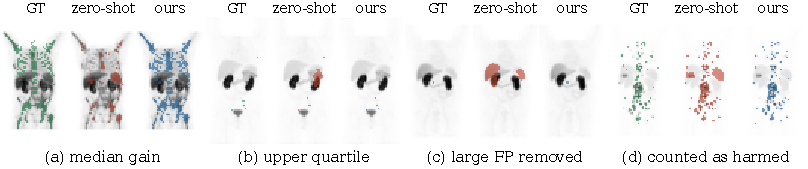
\includegraphics[width=\linewidth]{fig/fig_qual.pdf}
  \caption{\textbf{Locked test patients}, coronal PET maximum-intensity projections with ground truth (green), the zero-shot FDG segmenter (red) and the certified fine-tuned segmenter (blue).
  (a, b) Patients at the median and upper quartile of the Dice gain. (c) Physiological kidney uptake segmented as tumour zero-shot (862\,mL) and removed after certified fine-tuning. (d) One of the three patients counted as \emph{harmed}: Dice rises from 0.27 to 0.60 and FP volume falls from 314 to 3\,mL, yet 4 of 106 detected lesions are lost.}
  \label{fig:qual}
\end{figure*}

\begin{figure}[t]
  \centering
  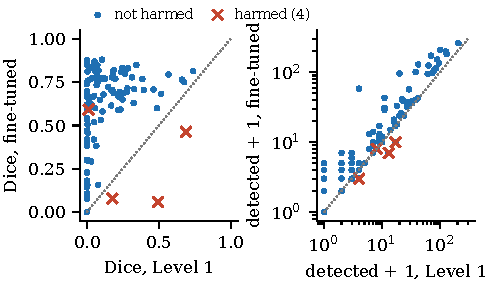
\includegraphics[width=\linewidth]{fig/fig_l2_B.pdf}
  \caption{\textbf{The Level-2 decision, on the certification set $\B$} (126 patients; the test set plays no part). Each point is a patient, Level-1 system ($x$) against fine-tuned segmenter ($y$). Left: Dice. Right: detected lesions (log scale, $+1$). Four patients are harmed (red): three lose detections, one loses Dice. Four of 126 cannot support a 5\% promise, so the switch is refused at $\delta=0.05$ and certified at $\delta=0.10$.}
  \label{fig:l2B}
\end{figure}

\subsection{Patient by patient}
\label{sec:patients}
Means hide what the certificate is about, so we look at every test patient (\cref{fig:patients}; descriptive, \cref{sec:setup}).

\para{Harm is invisible to the average.}
Naive self-improvement improves 49 patients by more than 0.01 Dice, worsens one, and still harms 11 (\cref{fig:patients}a).
All 11 lose lesions, and in 7 of them Dice \emph{rises} (by up to $+0.44$): removing a false-positive region that overlapped a lesion raises Dice and deletes the detection, and a mean-Dice criterion rewards exactly that.
Certified \ours improves 10 patients and harms none.

\para{Level 2 helps almost everyone.}
After certified fine-tuning (\cref{fig:patients}b,c) the median patient's Dice is 0.63, and 77 of 119 tumour-positive patients exceed 0.5 (5 before).
Lesion-level sensitivity rises from 46\% to 79\%: 1,460 detections are gained and 7 lost, all in the three harmed patients.
Two patients keep more than 100\,mL of false-positive volume (104 before).
\para{No subgroup is left behind.}
By radionuclide, scanner vendor and tumour burden (\cref{tab:subgroups}; full table in \cref{tab:supp_sub}), the gain ranges from $+0.36$ to $+0.49$ Dice with every interval above zero, and no subgroup has more than 2 harmed patients.
The weakest starting points gain most: vendor 1 (Level-1 Dice 0.06) and patients with one or two lesions (0.01) both reach about 0.5.
Harm, however, sits where the margin is thinnest: two of the three harmed patients have one or two lesions, where a single lost lesion is the patient's whole disease.
The residual false-positive volume is concentrated in the highest-burden patients (39\,mL per scan, against 2--4\,mL for patients with fewer lesions).

\begin{table}[t]
\centering
\caption{\textbf{Level 2 by subgroup} (locked $\C$, post hoc). Dice over tumour-positive patients, Level-1 system $\to$ certified fine-tuned segmenter; $\Delta$ with 95\% bootstrap interval; harmed relative to the Level-1 system. Vendors numbered by cohort size; burden in tertiles of lesion count.}
\label{tab:subgroups}
\footnotesize
\setlength{\tabcolsep}{3pt}
\begin{tabular}{@{}lcccc@{}}
\toprule
subgroup & $n$ & Dice & $\Delta$Dice {\scriptsize[95\% CI]} & harmed \\
\midrule
all & 125 & 0.116$\to$0.547 & $+0.431$ {\scriptsize[$+0.388$, $+0.475$]} & 3 \\
\midrule
$^{18}$F & 71 & 0.125$\to$0.551 & $+0.426$ {\scriptsize[$+0.376$, $+0.479$]} & 1 \\
$^{68}$Ga & 54 & 0.103$\to$0.541 & $+0.438$ {\scriptsize[$+0.361$, $+0.507$]} & 2 \\
vendor 1 & 55 & 0.061$\to$0.521 & $+0.460$ {\scriptsize[$+0.380$, $+0.532$]} & 2 \\
vendor 2 & 70 & 0.160$\to$0.568 & $+0.408$ {\scriptsize[$+0.357$, $+0.455$]} & 1 \\
1--2 lesions & 41 & 0.011$\to$0.453 & $+0.442$ {\scriptsize[$+0.348$, $+0.537$]} & 2 \\
3--24 lesions & 38 & 0.049$\to$0.543 & $+0.493$ {\scriptsize[$+0.434$, $+0.548$]} & 0 \\
$\ge$25 lesions & 40 & 0.286$\to$0.647 & $+0.361$ {\scriptsize[$+0.305$, $+0.416$]} & 1 \\
\bottomrule
\end{tabular}
\end{table}

\subsection{Does the conclusion depend on the harm definition?}
\label{sec:harmdef}
The harm event (\cref{eq:harm}) is a choice, fixed before any PSMA number was computed.
To see whether our conclusions rest on it, we recount harm for every locked arm under six alternatives (\cref{tab:harmdef}; post hoc, descriptive).
Two things hold under all of them.
Certified \ours harms no test patient.
And the Level-2 decision is unchanged: the fine-tuned segmenter harms 3 or 4 of the 126 certification patients, so it is refused at $\delta=0.05$ ($p\ge0.12>\alpha/2$) and certified at $\delta=0.10$ ($p\le0.004$).
Naive selection harms 11 patients whenever a single lost lesion counts, and still 5--7 when only larger losses do.

The instructive row is the Dice-only definition.
Under it naive selection harms a \emph{single} patient: a safety check based on segmentation overlap alone would see almost none of its harm, because it is lesion loss hidden inside a Dice gain (\cref{sec:patients}).
The opposite extreme, $\varepsilon=0$, counts numerical noise as harm: pseudo-labelling then ``harms'' 39 patients through Dice changes below 0.01.
One caveat: at Level 1 a different definition would also change \emph{which} updates certify on $\B$; the stored outputs of the locked arms cannot show that, so \cref{tab:harmdef} evaluates the decisions we made, not the decisions we would have made.

\begin{table}[t]
\centering
\caption{\textbf{Harm under alternative definitions} (post hoc). Harmed patients of each locked arm on $\C$ ($n=125$, Level-1 arms relative to $f_0$) and of the fine-tuned segmenter (FT) on $\B$ ($n=126$, with the Level-2 $p$-value at $\delta=0.05$; every definition gives $p\le0.004$ at $\delta=0.10$) and on $\C$, relative to the Level-1 system. ``Lost'': fewer ground-truth lesions detected than the reference.}
\label{tab:harmdef}
\footnotesize
\setlength{\tabcolsep}{2.6pt}
\begin{tabular}{@{}lccccc@{}}
\toprule
harm if \ldots & naive & pseudo & \ours & FT, $\B$ ($p$) & FT, $\C$ \\
\midrule
\textbf{lost $\ge$1 or $\Delta$Dice${<}{-}0.01$} & 11 & 4 & 0 & 4 (0.24) & 3 \\
lost $\ge$1 & 11 & 1 & 0 & 3 (0.12) & 3 \\
$\Delta$Dice${<}{-}0.01$ & 1 & 3 & 0 & 3 (0.12) & 2 \\
lost $\ge$1 or $\Delta$Dice${<}0$ & 11 & 39 & 0 & 4 (0.24) & 3 \\
lost $\ge$1 or $\Delta$Dice${<}{-}0.05$ & 11 & 1 & 0 & 4 (0.24) & 3 \\
lost $\ge$2 or $\Delta$Dice${<}{-}0.01$ & 5 & 3 & 0 & 3 (0.12) & 3 \\
lost ${>}10\%$ or $\Delta$Dice${<}{-}0.01$ & 7 & 3 & 0 & 4 (0.24) & 2 \\
\bottomrule
\end{tabular}
\end{table}

\begin{figure*}[t]
  \centering
  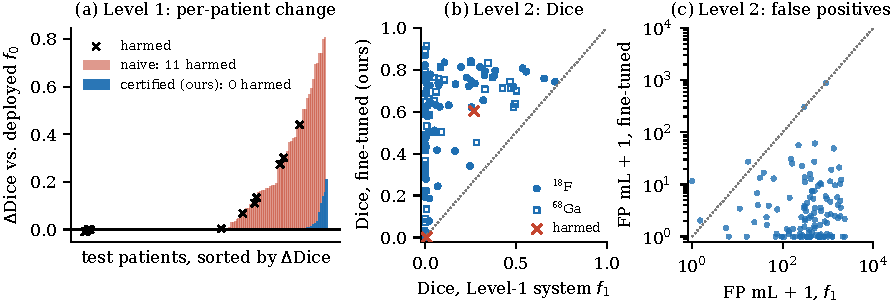
\includegraphics[width=\linewidth]{fig/fig_patients.pdf}
  \caption{\textbf{Every locked test patient.}
  (a) Level 1: per-patient Dice change relative to the deployed agent, sorted; $\times$ marks harmed patients. Naive selection harms 11 patients, all by lost lesions, 7 of them while \emph{raising} their Dice; certified \ours harms none.
  (b) Level 2: per-patient Dice of the Level-1 system and of the certified fine-tuned segmenter ($^{18}$F filled, $^{68}$Ga open; red $\times$: the three harmed patients).
  (c) Level 2: per-patient false-positive volume (log scale).}
  \label{fig:patients}
\end{figure*}

\subsection{Does the certificate keep its promise?}
\label{sec:validity}
A single test set is one draw.
To measure how often each selection rule breaks its promise, we resample the 251 patients of $\B\cup\C$ into 1,000 random halves, select on one half and measure the realised harm rate on the other, with detectors fixed.
\Cref{fig:validity} shows the violation frequency $\Pr[\hat R>\delta]$ at $\delta=0.05$.
Certified selection violates in 0.2--0.5\% of splits on all three segmentation backbones, within $\alpha=5\%$; naive selection violates in 98.5--99.6\%.
At $\delta=0.10$ the rates are 0.3--0.7\% against 35--52\%.
The same holds in the source domain: on 630 FDG patients, naive selection breaks a 2\% promise in 76.6\% of splits and certified selection in 0.8\%.
Naive selection is not merely riskier; its stated risk is wrong.

\begin{figure}[t]
  \centering
  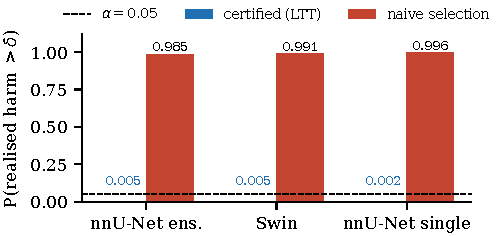
\includegraphics[width=\linewidth]{fig/fig_validity.pdf}
  \caption{\textbf{Validity.} Fraction of 1,000 random selection/evaluation splits of $\B\cup\C$ in which the realised harm rate exceeds the promised $\delta=0.05$, for three segmentation backbones.}
  \label{fig:validity}
\end{figure}

\subsection{The risk--benefit dial}
\label{sec:dial}
\Cref{fig:dial} sweeps the tolerance for the Level-1 agent updates, certifying on $\B$ and measuring on the locked $\C$.
At $\delta=0.03$ nothing is certifiable at $n=126$ (\cref{sec:ltt}) and the system rolls back; from $\delta=0.05$ to $0.20$ the summed benefit grows from $+0.79$ to $+4.63$ Dice-points, approaching naive selection ($+5.63$) while the realised harm rate stays below $\delta$ at every setting.
At Level 2 the dial is a step: rollback at $\delta=0.05$, the fine-tuned segmenter from $\delta=0.10$ on.
The dial does not tell a site which tolerance to choose; it tells it, before deployment, what each tolerance buys.

\para{The price of a guarantee.}
With 4 harmed of 126, the Level-2 switch is certifiable for any $\delta\ge0.080$ (\cref{fig:power}b).
The same 4 harms would certify $\delta=0.05$ among 202 certification patients; a 1\% guarantee needs at least 368 patients even if none is harmed (\cref{fig:power}a, \cref{tab:supp_n}).
A site can compute this cost before it labels a single case.

\begin{figure}[t]
  \centering
  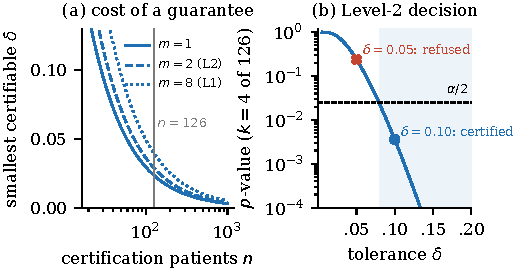
\includegraphics[width=\linewidth]{fig/fig_power.pdf}
  \caption{\textbf{The price of a guarantee.} (a) Smallest certifiable tolerance with zero observed harms, $1-(\alpha/m)^{1/n}$, against the number of certification patients, for $m$ chains ($\alpha=0.05$). (b) Level-2 $p$-value on $\B$ (4 of 126 patients harmed) against $\delta$; the switch is certified where $p\le\alpha/2$ (shaded).}
  \label{fig:power}
\end{figure}

\begin{figure}[t]
  \centering
  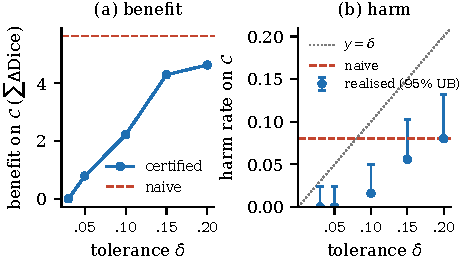
\includegraphics[width=\linewidth]{fig/fig_dial.pdf}
  \caption{\textbf{Risk--benefit dial} (Level 1, locked $\C$). (a) Summed Dice benefit of the certified update as the tolerance $\delta$ grows; naive selection dashed. (b) Realised harm rate with 95\% upper bound, against $y=\delta$. Computed from per-action outcomes rather than an end-to-end agent run, so the naive point harms 10 patients, not the 11 of \cref{tab:main}.}
  \label{fig:dial}
\end{figure}

\begin{table}[t]
\centering
\caption{\textbf{Generality across segmenters} (Level 1, locked $\C$, $\delta=0.05$). Benefit is relative to the deployed agent on the same segmenter. $\dagger$: safety not confirmed after the pre-registered Holm correction over the two secondary backbones ($p=0.048>0.025$).}
\label{tab:backbones}
\setlength{\tabcolsep}{3.4pt}
\small
\begin{tabular}{@{}lccc@{}}
\toprule
segmenter & harmed (UB) & $\Delta$Dice {\scriptsize[95\% CI]} & $\Delta$FP mL \\
\midrule
nnU-Net, 5-fold & 0 (2.4\%) & \makecell{$+0.0068$\\[-2pt]{\scriptsize[$+0.0022$, $+0.0126$]}} & $-127$ \\
Swin & 2 (5.0\%)$^\dagger$ & \makecell{$+0.0055$\\[-2pt]{\scriptsize[$+0.0011$, $+0.0123$]}} & $-163$ \\
nnU-Net, single & 2 (5.0\%)$^\dagger$ & \makecell{$+0.0012$\\[-2pt]{\scriptsize[$+0.0003$, $+0.0026$]}} & $-68$ \\
\bottomrule
\end{tabular}
\end{table}

\subsection{Generality across segmenters}
\label{sec:generality}
We repeat Level-1 certification on two further PSMA segmenters, a Swin-transformer backbone~\cite{liu2021swin} and a single nnU-Net model (\cref{tab:backbones}).
The Dice benefit and the FP reduction replicate on both ($p<0.001$ each).
Each harms 2 of 125 test patients (1.6\%, below $\delta$), but with the pre-registered Holm correction the safety endpoint is not confirmed on either, and each loses 2 lesion detections.
Validity (\cref{fig:validity}) holds on all three.
